\documentclass{report}
\usepackage{amsmath}
\usepackage{graphicx}
\usepackage{booktabs}

\title{Labwork 3: Hello, CUDA!}
\author{Nguyen Duy Anh Tung}
\date{\today}

\begin{document}
\maketitle

\section{Introduction}
In this labwork, we implement an RGB-to-grayscale image converter using both sequential CPU programming and GPU acceleration with Numba CUDA. The objective is to evaluate the speedup gained from parallel processing and examine how different thread block sizes affect execution time.

\section{Implementation}
The implementation consists of two parts:
\begin{itemize}
    \item \textbf{CPU Implementation}: Reads the image, flattens it to shape $(N, 3)$, and calculates the grayscale value pixel-by-pixel using a sequential loop with formula $g = \lfloor(R + G + B) / 3\rfloor$.
    \item \textbf{GPU Implementation}: Implements a CUDA kernel where each thread calculates its global index:
    \[
    \text{tidx} = \text{threadIdx.x} + \text{blockIdx.x} \times \text{blockDim.x}
    \]
    The input array is transferred to the GPU via \texttt{cuda.to\_device()}, computed in parallel, and the result is retrieved using \texttt{copy\_to\_host()}.
\end{itemize}

\section{Experimental Results}
Testing was conducted on an image containing $199,875$ pixels. The CPU execution time was \textbf{0.1577 s} ($157.7\text{ ms}$).

\begin{table}[htbp]
\centering
\begin{tabular}{rrrrr}
\toprule
\textbf{Block Size} & \textbf{Grid Size} & \textbf{GPU Time (ms)} & \textbf{Speedup} \\
\midrule
32   & 6247 & 0.17 & 906.1$\times$ \\
64   & 3124 & 0.17 & 903.6$\times$ \\
128  & 1562 & 0.16 & 964.2$\times$ \\
256  & 781  & 0.13 & 1198.2$\times$ \\
512  & 391  & 0.13 & 1231.7$\times$ \\
1024 & 196  & 0.13 & 1243.3$\times$ \\
\bottomrule
\end{tabular}
\caption{Performance comparison across different block sizes}
\end{table}

\begin{figure}[htbp]
\centering
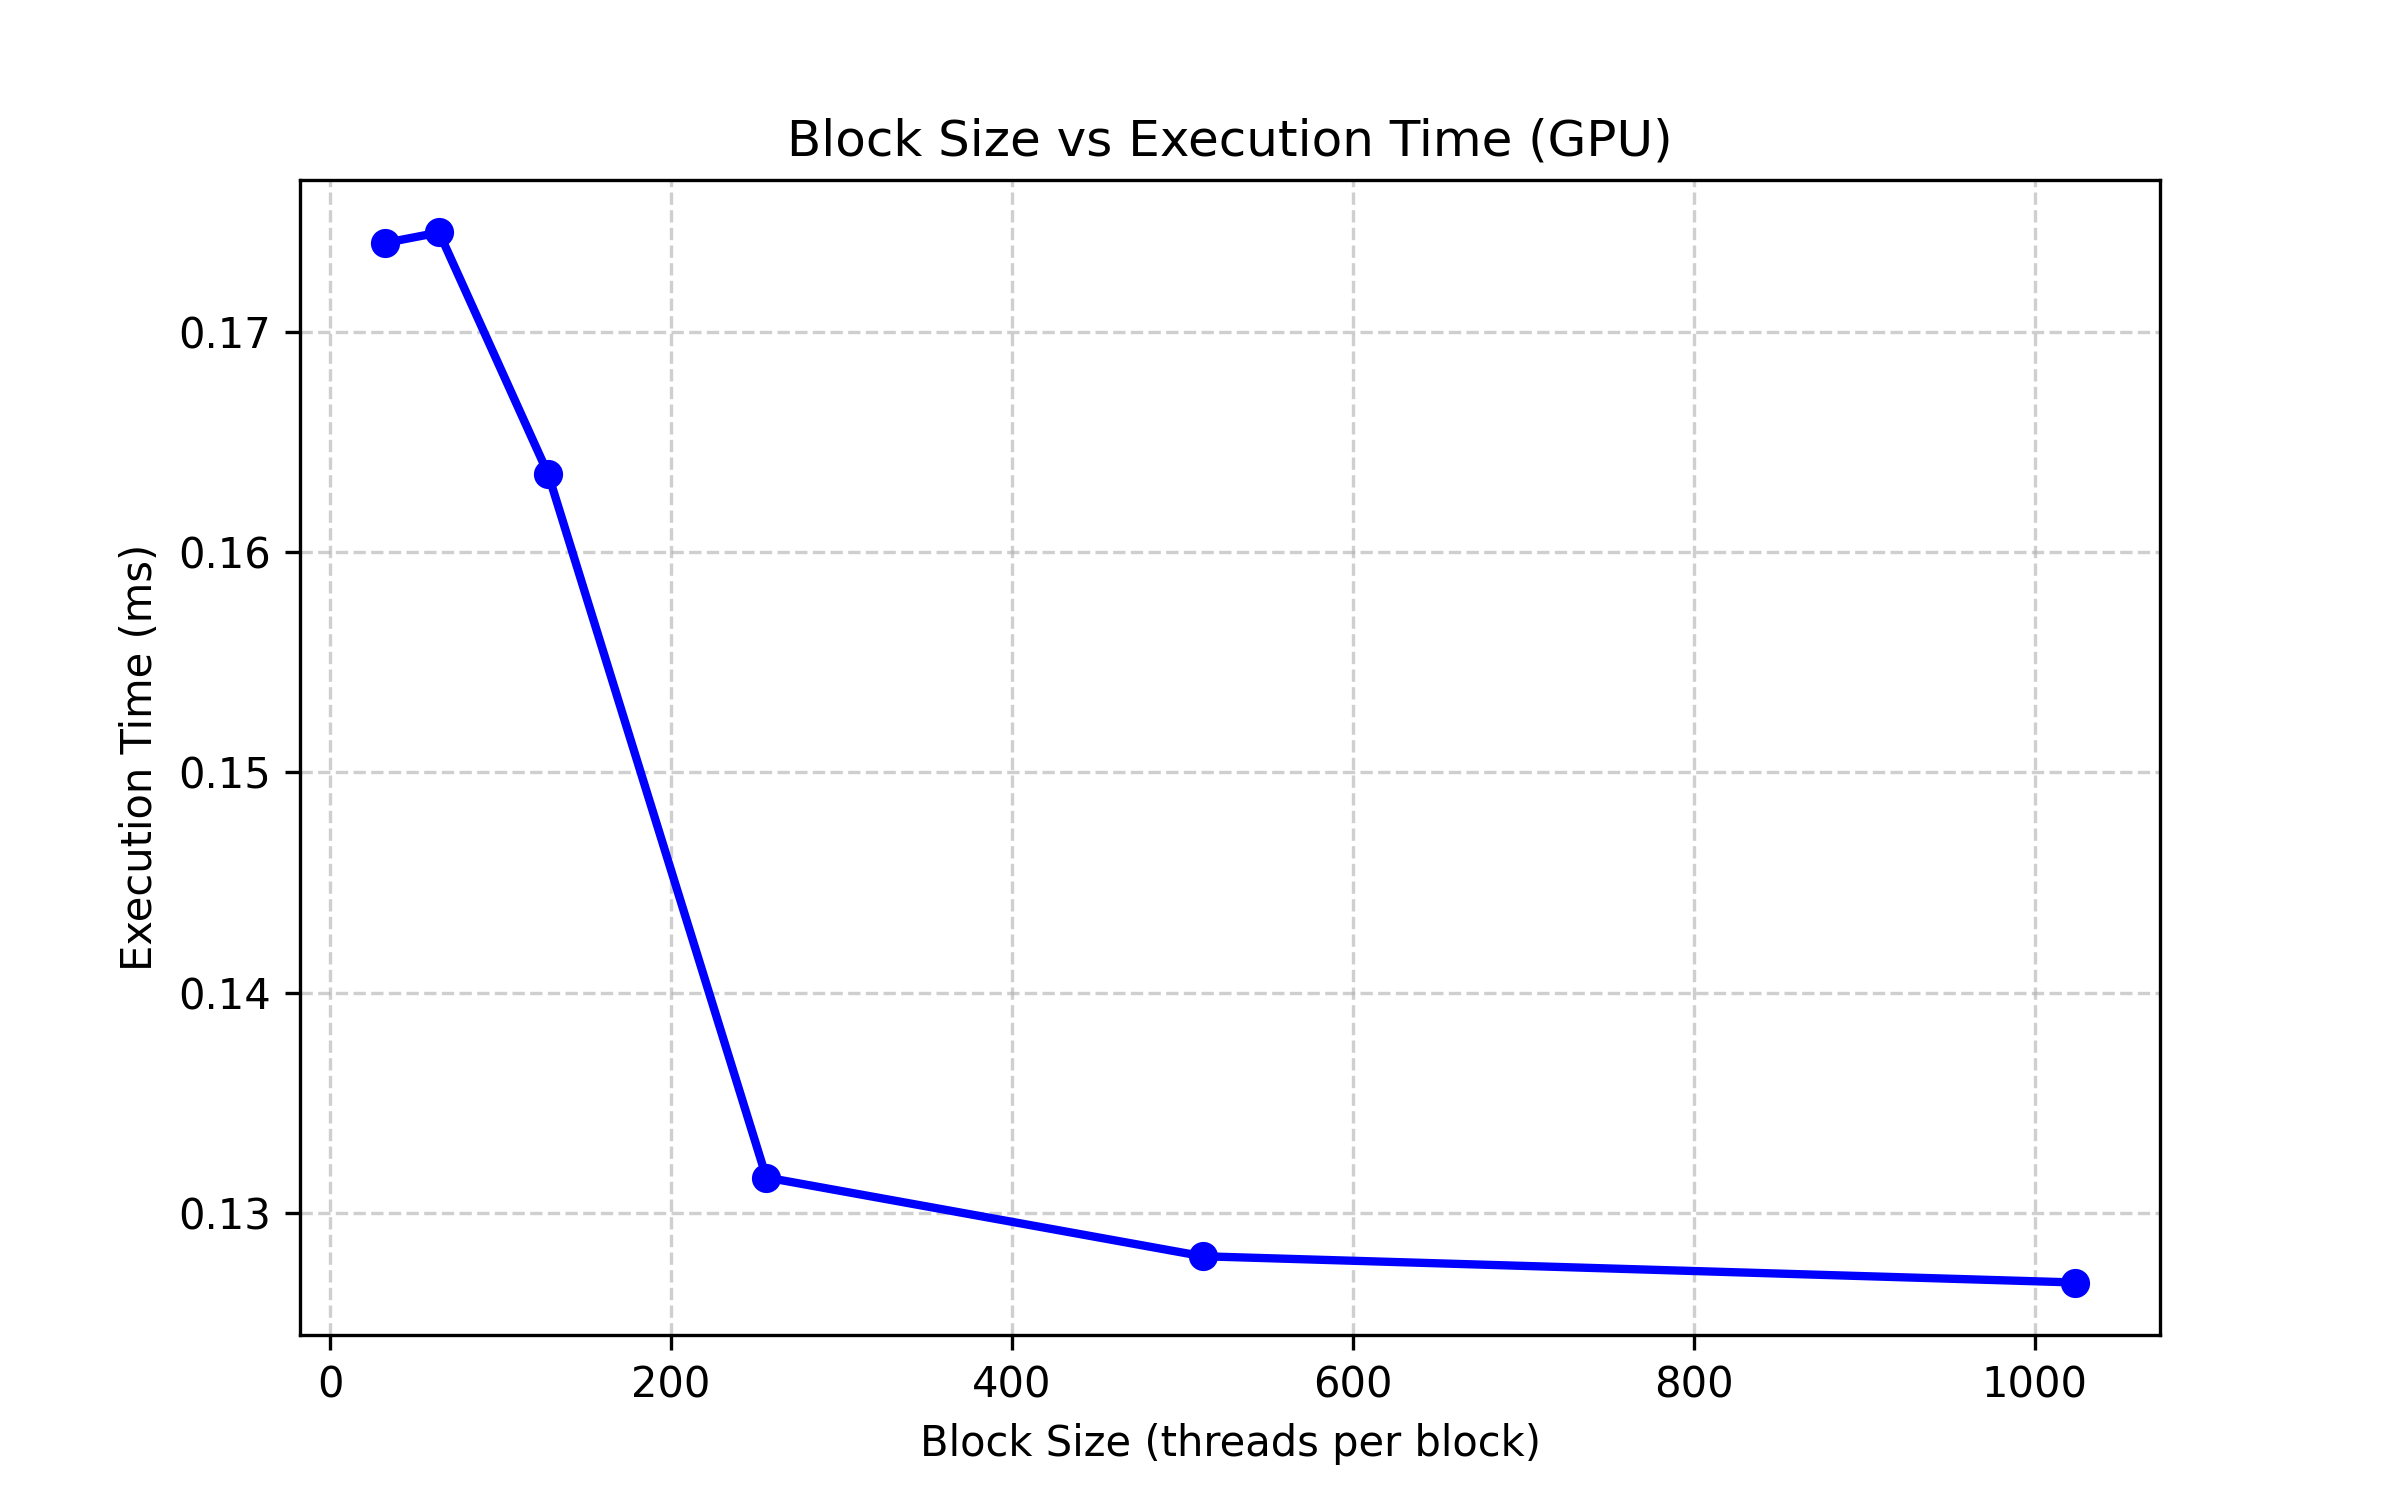
\includegraphics[width=0.8\textwidth]{block_size_vs_time.png}
\caption{Block size vs Execution Time on GPU}
\end{figure}

\section{Discussion}
\begin{itemize}
    \item \textbf{Speedup}: The GPU implementation achieves massive speedups ranging from $903.6\times$ to $1243.3\times$ compared to the sequential CPU execution.
    \item \textbf{Block Size Impact}: Increasing block size from 32 to 256 threads reduces kernel latency from $0.17\text{ ms}$ down to $0.13\text{ ms}$ due to fewer blocks needing to be scheduled. Beyond 256 threads (512 and 1024), execution time stabilizes at around $0.13\text{ ms}$, indicating that occupancy has saturated for this problem size.
\end{itemize}

\end{document}